% ---------------------------------------------------------------
% FOR OVERLEAF SUBMISSION (Springer LNCS / CLAIO2026):
%   Replace the next two lines with:
%     \documentclass[runningheads]{llncs}
%   Overleaf has llncs.cls pre-installed.
%   Remove \usepackage[margin=1in]{geometry} and the \maketitle redefinitions below.
% ---------------------------------------------------------------
\documentclass[11pt,a4paper]{article}

% ---------------------------------------------------------------
% Core packages
% ---------------------------------------------------------------
\usepackage[T1]{fontenc}
\usepackage[utf8]{inputenc}
\usepackage[margin=1in]{geometry}
\usepackage{graphicx}
\usepackage{booktabs}
\usepackage{amsmath,amssymb}
\usepackage{siunitx}
\usepackage[font=small,labelfont=bf]{caption}
\usepackage{subcaption}
\usepackage[colorlinks=true,linkcolor=black,citecolor=black,urlcolor=black]{hyperref}
\usepackage[capitalise,nameinlink]{cleveref}
% \usepackage{microtype}  % enable on Overleaf; requires scalable fonts locally
\usepackage{multirow}
\usepackage{array}
\usepackage{tabularx}
\usepackage{xcolor}
\usepackage{url}
\usepackage[ruled,vlined]{algorithm2e}
\usepackage{parskip}
\setlength{\parskip}{4pt}

% ---------------------------------------------------------------
% siunitx settings
% ---------------------------------------------------------------
\sisetup{
  table-number-alignment = center,
  detect-weight = true
}

% ---------------------------------------------------------------
% Stub commands for LNCS compatibility
% (delete when switching to llncs.cls on Overleaf)
% ---------------------------------------------------------------
\newcommand{\institute}[1]{\def\@institute{#1}}
\newcommand{\titlerunning}[1]{}
\newcommand{\authorrunning}[1]{}
\newenvironment{keywords}{\par\smallskip\noindent\textbf{Keywords:} }{\par}

% ---------------------------------------------------------------
% Path for figures
% ---------------------------------------------------------------
\graphicspath{{figures/}}

% ---------------------------------------------------------------
\begin{document}

\title{\textbf{A Graph-Based Geospatial Optimization Framework\\
       for Retail Branch Expansion:\\[4pt]
       Calibration, Baseline Comparison, and Cross-Context Validation}}

\author{[Author names anonymized for review]\\
        \small [Institution anonymized for review]}

\date{}
\maketitle

% ---------------------------------------------------------------
\begin{abstract}
Facility location decisions in dense urban environments depend not only on
population size but also on network accessibility, territorial structure,
and socioeconomic heterogeneity. This paper presents a modular geospatial
optimization framework that integrates pedestrian-network distances derived
from OpenStreetMap, graph-based spectral clustering, multiple correspondence
analysis~(MCA), and a clustered \mbox{p-median} formulation with coverage,
separation, and demand-penalty constraints.
The methodological contribution is a complete, calibrated pipeline in which
every parameter is justified through multi-objective sensitivity
analysis over an 81-point grid rather than fixed \textit{a priori}.
A proportional-demand allocation rule replaces the original fixed-per-cluster
budget, reducing inequity across territories of different size.

The framework is validated across three urban contexts in Mexico that differ
substantially in density, infrastructure supply, and commercial maturity:
a dense student-area district (Tecnológico de Monterrey, Monterrey),
a less-developed city~(Villahermosa, Tabasco), and an industrial
corridor~(Estado de México).
In all three settings the clustered model is compared on equal terms against
four baselines evaluated under pedestrian-network distance:
a global \mbox{p-median} optimum, a \mbox{k-means} partitioning baseline,
an Euclidean-solve baseline, and a no-MCA variant.
The proposed model retains \SIrange{93.2}{99.9}{\percent} of the global
optimum coverage while reducing solver runtime by up to \SI{67}{\percent}
in larger instances.
Euclidean-distance models underestimate mean assignment distance by
\SIrange{10}{20}{\percent} relative to network evaluation, confirming
that pedestrian routing is an essential component of any urban
accessibility assessment.
The framework is modular and transferable to clinics, pharmacies,
service offices, and other location systems where
network accessibility and territorial heterogeneity are primary concerns.

\end{abstract}

\begin{keywords}
facility location $\cdot$ p-median $\cdot$ spectral clustering $\cdot$
multiple correspondence analysis $\cdot$ geospatial optimization $\cdot$
retail analytics $\cdot$ parameter calibration
\end{keywords}

% ---------------------------------------------------------------
\section{Introduction}
\label{sec:intro}

Retail expansion in urban areas involves a class of decisions that is structurally
different from classical facility location in two important respects.
First, the set of feasible locations is heterogeneous: some blocks are already
served by existing stores, some lack the pedestrian connectivity needed to
attract walk-in traffic, and some exhibit socioeconomic profiles that make
demand volumes hard to estimate from population counts alone.
Second, operational constraints—minimum separation between openings,
service radii calibrated to walking time, and budget limits allocated
across operating territories—impose combinatorial structure that Euclidean
approximations cannot capture faithfully.

Classical \mbox{p-median} models minimize total demand-weighted assignment
distance~\cite{hakimi1964optimum} and have been applied extensively to
retail, public facility, and logistics network design~\cite{daskin1995network,%
tadic2023locating}.
However, in practice these models are typically deployed at a scale where
solving a single global instance is computationally tractable, and their
demand weights are constructed from scalar population counts that discard
qualitative urban-environment information.
The contribution of this work is a computational framework that addresses
both limitations simultaneously.

The pipeline combines four layers:
(\textit{i})~a pedestrian street network derived from
OpenStreetMap~\cite{osm2025} and processed with OSMnx~\cite{boeing2017osmnx},
which replaces Euclidean proximity with shortest-path distance to
capture real access effort;
(\textit{ii})~graph-based spectral clustering~\cite{ng2002spectral,%
vonluxburg2007tutorial}, which partitions the study area into operationally
coherent territories by exploiting road-network affinity rather than
Euclidean geometry;
(\textit{iii})~multiple correspondence analysis~(MCA)~\cite{greenacre2017correspondence},
which compresses 33 categorical socio-urban census indicators into a single
interpretable demand modifier; and
(\textit{iv})~a \mbox{p-median} model solved independently in each cluster
with coverage-radius, minimum-separation, and uncovered-demand-penalty
constraints.

A key methodological addition relative to the original formulation is
\textit{parameter calibration through multi-objective sensitivity analysis}.
The service radius~$D_{\max}$, the MCA weight~$\beta$, and the candidate-block
threshold are jointly optimized over an 81-point Pareto grid rather than
fixed by convention.
A second addition is a \textit{demand-proportional budget allocation} rule that
distributes the total opening budget across clusters according to their
weighted demand share, removing the fixed-seven-per-cluster rule that generated
artificial inequity in the original submission.

The framework is validated across three urban contexts in Mexico that differ
substantially in commercial maturity and spatial density, and is compared
against four baselines—all evaluated under consistent pedestrian-network
distance—to allow fair performance attribution.

The main contributions of this paper are:
\begin{itemize}
  \item A calibrated, parameter-justified facility-location pipeline in which
        $D_{\max}$, $\beta$, and the candidate threshold are selected from
        a Pareto-optimal grid search rather than set \textit{a priori}
        (\cref{sec:methodology}).
  \item A demand-proportional cluster-budget allocation rule that replaces
        the fixed-per-cluster opening count and reduces inter-cluster
        coverage inequity (\cref{sec:methodology}).
  \item A rigorous baseline comparison that isolates the contribution of
        network distances, spectral clustering, and MCA weighting through
        four controlled variants, all evaluated under pedestrian-network
        distance (\cref{sec:experiments}).
  \item A cross-context validation across three urban settings that exhibit
        qualitatively different store-supply densities and street
        connectivity patterns (\cref{sec:experiments}).
  \item Empirical evidence that coverage loss from territorial decomposition
        remains below~$7$\% in all tested instances, and that Euclidean-solve
        models underestimate mean assignment distance by up to~$20$\%
        relative to network evaluation (\cref{sec:results}).
\end{itemize}

\section{Related Work}
\label{sec:related}

\paragraph{Network facility location.}
The \mbox{p-median} problem seeks to select $p$ service sites that minimize
total demand-weighted assignment distance~\cite{hakimi1964optimum}.
Its network variant, in which distances are shortest paths on a graph rather
than Euclidean measures, is the natural model when travel effort matters.
Maranzana's early observation that Euclidean distances understate network
costs in irregular urban street layouts~\cite{maranzana1964siting} has been
confirmed repeatedly in empirical studies; Boeing's OSMnx library has made
pedestrian-network extraction operationally straightforward~\cite{boeing2017osmnx}.
Solution methods for medium-to-large instances range from Lagrangian relaxation
and column generation to commercial MILP
solvers~\cite{avella2007lagrangian,lorena2003constructive}.
For instances with thousands of candidate sites and demand nodes,
decomposition approaches that reduce the effective problem size have
practical value, as long as the decomposition does not introduce large
coverage gaps relative to the global optimum.

\paragraph{Clustering-based territorial decomposition.}
Partitioning a study area before solving a subproblem independently in each
territory is a well-known heuristic for scaling facility location to larger
instances.
The quality of the decomposition depends on whether the partition respects
the connectivity of the underlying network.
Centroid-based methods such as \mbox{k-means} impose Euclidean distances on
both the partition and the assignment, which introduces inconsistency when
actual travel distances are non-Euclidean.
Spectral clustering~\cite{shi2000normalized,ng2002spectral,vonluxburg2007tutorial}
avoids this by using the normalized graph Laplacian of an affinity matrix
defined on road-network distances; the resulting partition follows the
connectivity structure of the street network rather than Euclidean geometry.
The eigengap heuristic provides a data-driven criterion for selecting the
number of clusters, and a silhouette-score secondary check supplies additional
validation~\cite{theodoridis2009clustering}.
A post-processing merge rule that absorbs small territories into their nearest
major cluster bridges the gap between the mathematically selected partition
and the operationally deployable territory count.

\paragraph{Socioeconomic demand weighting.}
Demand models in urban facility location typically scale by population count,
which disregards heterogeneity in purchasing power, infrastructure quality,
and transport access.
MCA provides a principled method for compressing multiple categorical census
variables into orthogonal latent dimensions~\cite{greenacre1988correspondence,%
greenacre2006multiple,greenacre2017correspondence}.
Because census data are inherently categorical or categorized, MCA is preferable
to PCA: it operates on the indicator matrix of dummy-coded categories rather
than on a covariance matrix of continuous variables.
Greenacre's corrected-inertia formula removes the inflation that raw MCA
eigenvalues exhibit when the number of indicator columns is large, making
dimension importance comparable across models~\cite{greenacre1991interpreting}.
The normalized first MCA dimension serves as a socio-urban quality gradient
that upweights blocks with better infrastructure, education, and housing
services, directing new openings toward areas where economic activity
is most likely to be sustained.

\paragraph{Gap in existing work.}
Prior applications of \mbox{p-median} models to convenience-store or retail
location typically fix parameters by convention, use Euclidean distances as
a proxy, compare against no baseline, and validate in a single geographic
context.
This paper addresses all four gaps: parameters are calibrated from data,
distances are pedestrian-network distances in both solving and evaluation,
four controlled baselines are compared on equal terms, and the framework
is validated in three urban settings with qualitatively different
supply-demand structures.

\section{Methodology}
\label{sec:methodology}

The framework proceeds through five sequential stages:
candidate generation, spectral clustering, MCA-based demand weighting,
proportional budget allocation, and clustered \mbox{p-median} optimization.
Each stage is described below, together with the design rationale
that distinguishes each algorithmic choice from simpler alternatives.

% ---------------------------------------------------------------
\subsection{Pedestrian Network and Candidate Generation}
\label{ssec:network}

All distance computations are performed on the pedestrian street network
downloaded from OpenStreetMap~\cite{osm2025} and processed with
OSMnx~\cite{boeing2017osmnx}.
Census-block centroids and existing store locations are snapped to their
nearest graph node before shortest-path computation.
Let $G = (V, E)$ denote the projected walking graph and let $d_{u,v}$
be the shortest-path distance between nodes $u, v \in V$.

The first screening stage identifies blocks that are potentially underserved
by the existing store network.
For each census block~$i$, let $\delta_i$ denote its shortest-path distance
to the nearest existing store.
A block is classified as a \emph{candidate} if
\begin{equation}
  \delta_i > \tau \cdot \bar{d}_{\text{nn}},
  \label{eq:threshold}
\end{equation}
where $\bar{d}_{\text{nn}}$ is the empirical average nearest-neighbor distance
among all existing stores and $\tau$ is a multiplier calibrated from data.
Setting $\tau = 1.0$—so that the threshold matches the observed inter-store
spacing—produces a candidate set whose size is directly tied to the
existing coverage density rather than to an arbitrary absolute cutoff.
Sensitivity of coverage rate to $\tau \in \{0.5, 0.75, 1.0, 1.25, 1.5\}$
is reported in \cref{sec:sensitivity}.

% ---------------------------------------------------------------
\subsection{Graph-Based Spectral Clustering}
\label{ssec:spectral}

Computing all-pairs pedestrian distances is impractical for large instances.
Instead, a sparse affinity matrix is constructed in two steps.
For each census block, the $K = 12$ nearest neighbors in Euclidean space are
identified; for those candidate pairs only, the actual road-network distance
is computed.
The affinity between blocks $i$ and $j$ is defined by a Gaussian kernel:
\begin{equation}
  w_{i,j} = \exp\!\left(-\frac{d_{i,j}^{2}}{2\sigma^{2}}\right),
  \label{eq:affinity}
\end{equation}
where $\sigma$ is the median observed road-network distance among all evaluated
neighbor pairs.
The resulting sparse matrix $W$ defines a weighted similarity graph
whose edges reflect actual network connectivity rather than geometric proximity.

The normalized graph Laplacian is:
\begin{equation}
  L = D^{-1/2}(D - W)D^{-1/2},
  \label{eq:laplacian}
\end{equation}
where $D$ is the diagonal degree matrix of $W$.
The initial cluster count $k^*$ is selected by the eigengap heuristic:
\begin{equation}
  k^* = \arg\max_k \left(\lambda_{k+1} - \lambda_k\right),
  \label{eq:eigengap}
\end{equation}
using the smallest eigenvalues of $L$~\cite{vonluxburg2007tutorial}.
\Cref{fig:eigengap} shows the eigenvalue spectrum and eigengap profile
for the student-area instance ($k^* = 16$); the result is confirmed by a
secondary silhouette analysis (\cref{fig:silhouette}).

The raw partition typically contains several very small territories.
To produce operationally deployable regions, clusters with fewer than
200 census blocks are merged into the nearest major cluster using
road-network distance whenever available and Euclidean distance as a fallback.
\Cref{fig:clusters} compares the raw $k^*$-cluster partition against
the final merged solution for the student-area instance.

The $K = 12$ neighbor count was validated by comparing eigengap stability
across $K \in \{6, 8, 10, 12, 15, 18\}$: lower values produce less stable
eigengaps and more fragmented clusters, while the signal is consistent
for $K \geq 12$ (\cref{fig:k_sensitivity}).

\begin{figure}[t]
  \centering
  \begin{subfigure}[b]{0.49\textwidth}
    
\includegraphics[width=\textwidth]{spectral_eigengap_decision}
    \caption{Eigenvalue spectrum and eigengap ($k^*=16$, student area).}
    \label{fig:eigengap}
  \end{subfigure}\hfill
  \begin{subfigure}[b]{0.49\textwidth}
    
\includegraphics[width=\textwidth]{spectral_silhouette_support}
    \caption{Silhouette coefficient for $k$ values around $k^*$.}
    \label{fig:silhouette}
  \end{subfigure}
  \caption{Spectral cluster-count selection for the student-area instance.
           The eigengap selects $k^*=16$; silhouette analysis provides
           secondary confirmation.}
  \label{fig:cluster_selection}
\end{figure}

\begin{figure}[t]
  \centering
  
\includegraphics[width=\textwidth]{graph_spectral_clusters_before_after_merge}
  \caption{Raw 16-cluster partition (left) and the six-cluster solution
           after the small-cluster merge rule (right) for the student area.
           Road-network affinity preserves urban connectivity; the merge rule
           converts fragmented micro-territories into deployment-ready zones.}
  \label{fig:clusters}
\end{figure}

% ---------------------------------------------------------------
\subsection{Socio-Urban Demand Weighting via MCA}
\label{ssec:mca}

Population count alone is an insufficient demand proxy for retail location
because blocks of equal population can differ sharply in infrastructure quality,
transport access, and economic activity.
MCA is used instead of PCA because the source variables are categorical
or categorized~\cite{greenacre2017correspondence,greenacre2006multiple}.
Each continuous block-level variable is discretized into quintiles when
it has sufficient cardinality; otherwise, original categories are retained.
Missing values are explicitly encoded as an additional category so that
no observation is discarded.
The final indicator matrix contains 102 dummy columns derived from
33 source variables covering age structure, disability, schooling,
housing conditions, household services, and urban infrastructure
(street signage, bicycle lanes, pedestrian crossings, ramps,
public lighting, collective transport, and trees).

The resulting MCA coordinates are denoted $\text{MCA}_1, \text{MCA}_2, \ldots$
After Greenacre's correction~\cite{greenacre1991interpreting},
$\text{MCA}_1$ explains approximately 72\% of adjusted inertia
in the student-area instance (\cref{fig:mca_inertia}).
Infrastructure and urban-environment indicators---street signage, bicycle
infrastructure, pedestrian crossings, ramps, transport access, education,
and housing services---load most strongly on this dimension.
Categories reflecting higher schooling and more complete urban infrastructure
appear on the positive end of $\text{MCA}_1$, making it interpretable as a
socio-urban quality gradient rather than a purely demographic axis.

To prevent arbitrary sign from entering the optimization weights,
$\text{MCA}_1$ is oriented so that higher schooling corresponds to
positive values; if the raw extraction is inverted, all scores are
multiplied by $-1$.
The normalized demand modifier is then:
\begin{equation}
  \tilde{m}_i =
    \frac{\text{MCA}_{1,i} - \min(\text{MCA}_1)}
         {\max(\text{MCA}_1) - \min(\text{MCA}_1)},
  \label{eq:mca_norm}
\end{equation}
which rescales the gradient to $[0, 1]$ without altering relative differences.
\Cref{fig:mca_maps} confirms that $\text{MCA}_1$ scores exhibit strong
spatial continuity, which validates their use as a geographically structured
demand modifier.
\Cref{fig:mca_by_cluster} shows that spectral clusters differ not only
in geometry but also in their MCA profiles, reinforcing the rationale
for solving the optimization model within each territory independently.

\begin{figure}[t]
  \centering
  \begin{subfigure}[b]{0.49\textwidth}
    
\includegraphics[width=\textwidth]{mca_explained_components}
    \caption{Raw and Greenacre-corrected explained inertia by component.}
    \label{fig:mca_inertia}
  \end{subfigure}\hfill
  \begin{subfigure}[b]{0.49\textwidth}
    
\includegraphics[width=\textwidth]{mca_dims_by_cluster_boxplot}
    \caption{MCA\textsubscript{1,2,3} by spatial cluster.}
    \label{fig:mca_by_cluster}
  \end{subfigure}
  \caption{MCA component structure and its relationship to the spectral
           territory partition. The first corrected dimension concentrates
           most of the socio-urban variation; clusters differ in MCA profile
           as well as in spatial extent.}
  \label{fig:mca_structure}
\end{figure}

\begin{figure}[t]
  \centering
  
\includegraphics[width=\textwidth]{mca123_spatial_maps}
  \caption{Choropleth maps of $\text{MCA}_1$ (left), $\text{MCA}_2$ (center),
           and $\text{MCA}_3$ (right) for the student-area instance.
           The strong spatial continuity of $\text{MCA}_1$ validates its
           role as a geographically structured demand weight.}
  \label{fig:mca_maps}
\end{figure}

% ---------------------------------------------------------------
\subsection{Demand-Proportional Budget Allocation}
\label{ssec:allocation}

The original formulation allocated a fixed number of new openings ($p_{\text{new}}$)
to each cluster regardless of its size or demand.
In a six-cluster partition where cluster sizes range from 212 to 1,448 blocks
(\cref{tab:allocation}), a fixed allocation of seven openings per cluster
implies radically different per-demand coverage ratios across territories.
The largest cluster receives one opening per 184 blocks; the smallest,
one per 30.

To correct this, a proportional allocation rule is introduced:
\begin{equation}
  p_c = \max\!\left(1,\; \left\lfloor
    P_{\text{total}} \cdot \frac{\sum_{i \in C_c} w_i}
                                {\sum_{i \in I} w_i}
  \right\rceil\right),
  \label{eq:proportional}
\end{equation}
where $C_c$ is the set of demand blocks in cluster~$c$, $w_i$ is the
demand weight defined in \cref{eq:demand_weight} below,
and the allocation is rounded to the nearest integer with a minimum of one.
Integer remainder is distributed to the largest cluster.
\Cref{fig:allocation} shows the shift from fixed to proportional allocation
for all three study areas; the largest clusters receive substantially more
openings, which translates into measurable coverage gains in
blocks-per-opening terms.

\begin{table}[t]
  \centering
  \caption{Demand-proportional budget allocation versus the original
           fixed-per-cluster rule (student-area instance).}
  \label{tab:allocation}
  \begin{tabular}{rrrrrrr}
\toprule
\textbf{Cluster}
  & \textbf{Demand nodes}
  & \textbf{Population}
  & \textbf{Demand share (\%)}
  & \textbf{Fixed alloc.}
  & \textbf{Prop.\ alloc.} \\
\midrule
0 & 1{,}282 & 112{,}486 & 27.4 & 7 & 11 \\
1 & 1{,}182 & 102{,}309 & 25.1 & 7 & 11 \\
2 & 1{,}107 &  95{,}921 & 23.2 & 7 & 10 \\
3 &   590 &  49{,}175 & 11.9 & 7 &  5 \\
4 &   358 &  30{,}732 &  7.5 & 7 &  3 \\
5 &   212 &  19{,}836 &  4.9 & 7 &  2 \\
\midrule
\textbf{Total} & \textbf{4{,}731} & \textbf{410{,}459} & \textbf{100.0}
  & \textbf{42} & \textbf{42} \\
\bottomrule
\end{tabular}

\end{table}

\begin{figure}[t]
  \centering
  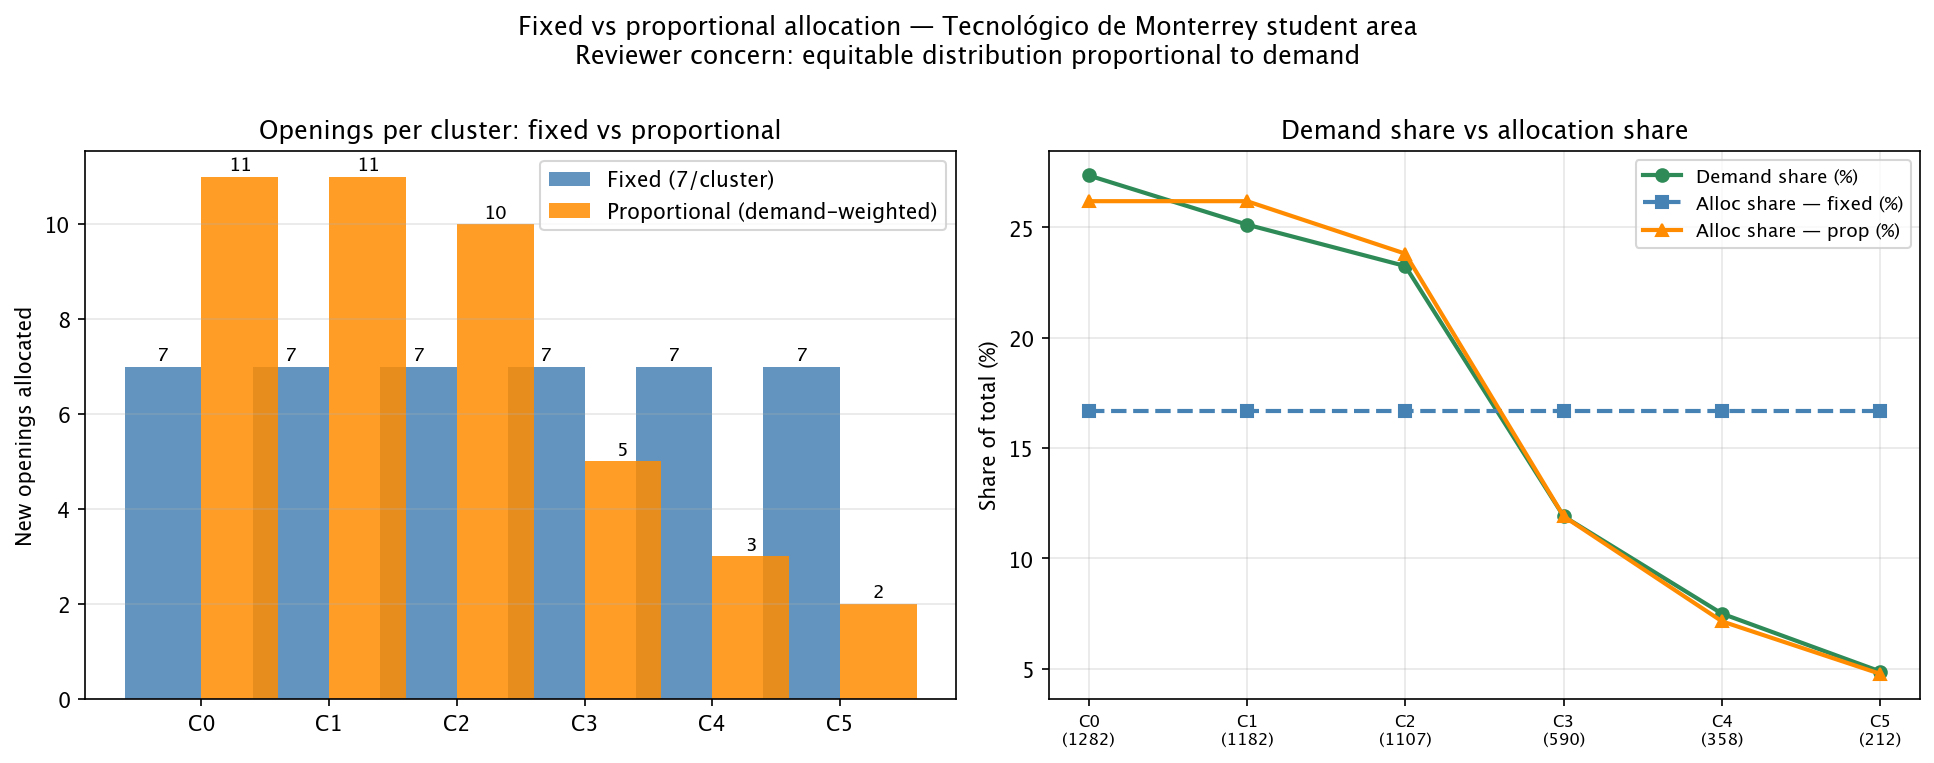
\includegraphics[width=0.7\textwidth]{fixed_vs_proportional_allocation}
  \caption{Fixed (original) versus proportional (revised) opening allocation
           by cluster for the student-area instance. The proportional rule
           concentrates the budget where demand is heaviest.}
  \label{fig:allocation}
\end{figure}

% ---------------------------------------------------------------
\subsection{Clustered P-Median Formulation}
\label{ssec:pmedian}

For each cluster $c$ the model is solved independently.
Let $I_c$ and $J_c$ denote the demand blocks and candidate sites
within cluster~$c$, let $E_c$ be the existing stores whose service
radii overlap with~$I_c$, and let $P_c = E_c \cup J_c$.
For each demand block~$i$, let $P_i = \{p \in P_c : d_{i,p} \leq D_{\max}\}$
be the set of feasible service points.
Let $\mathcal{C}_c \subset J_c \times J_c$ be the set of candidate pairs
separated by less than $S_{\min}$ (the minimum separation constraint
that prevents demand cannibalization).

The demand weight for block~$i$ is:
\begin{equation}
  w_i = p_i (1 + \beta \tilde{m}_i),
  \label{eq:demand_weight}
\end{equation}
where $p_i$ is the population of block~$i$ and $\beta \geq 0$ controls
the influence of the MCA modifier.
Setting $\beta = 0$ reduces the model to pure population weighting;
sensitivity to $\beta \in \{0.0, 0.1, 0.25, 0.5, 1.0\}$ is analyzed in
\cref{sec:sensitivity}.

Binary decision variables are:
$x_{i,p} = 1$ if block~$i$ is assigned to service point~$p$;
$y_j = 1$ if candidate~$j$ is opened; and
$u_i = 1$ if block~$i$ remains uncovered.
The objective minimizes total weighted assignment distance plus a penalty
for uncovered demand:
\begin{equation}
  \min \sum_{i \in I_c} \sum_{p \in P_i} w_i d_{i,p} x_{i,p}
       + \lambda \sum_{i \in I_c} w_i u_i.
  \label{eq:objective}
\end{equation}
Subject to:
\begin{align}
  \sum_{p \in P_i} x_{i,p} + u_i &= 1, && \forall i \in I_c,
  \label{eq:assignment} \\
  \sum_{j \in J_c} y_j &= p_c,
  \label{eq:budget} \\
  y_j + y_k &\leq 1, && \forall (j, k) \in \mathcal{C}_c,
  \label{eq:separation} \\
  x_{i,j} &\leq y_j, && \forall i \in I_c,\; j \in J_c \cap P_i,
  \label{eq:implication}
\end{align}
with $x_{i,p}, y_j, u_i \in \{0, 1\}$.
All subproblems are solved to optimality in the reported experiments
(\cref{sec:results}).

% ---------------------------------------------------------------
\subsection{Parameter Calibration}
\label{ssec:calibration}

A key weakness of the original submission was that parameters
$D_{\max}$, $S_{\min}$, $\beta$, and $\tau$ were fixed without empirical
justification.
This paper calibrates them jointly through a Pareto-frontier grid search
over 81 combinations of $D_{\max} \in \{300, 366, 450\}$~m,
$S_{\min} \in \{200, 240, 300\}$~m, and $p_c \in \{5, 7, 9\}$
per cluster (for three budget levels), repeated for
$\beta \in \{0.1, 0.25, 0.5\}$.

The Pareto criterion jointly optimizes coverage rate and weighted mean
assignment distance; parameter combinations on the frontier
are identified as calibration candidates.
The chosen parameters are selected from the frontier as those maximizing
coverage without simultaneously increasing weighted distance
beyond the frontier's convex hull (\cref{fig:pareto}).
\Cref{tab:parameters} reports the calibrated values for each study area.

\begin{table}[t]
  \centering
  \caption{Calibrated model parameters by study area.
           All values were selected from the Pareto grid rather than
           fixed \textit{a priori}.}
  \label{tab:parameters}
  \begin{tabular}{lllll}
\toprule
\textbf{Parameter} & \textbf{Meaning}
  & \textbf{Student} & \textbf{City} & \textbf{Industrial} \\
\midrule
$D_{\max}$ (m)
  & Service radius
  & 300 & 366 & 450 \\
$S_{\min}$ (m)
  & Min.\ candidate separation
  & 200 & 200 & 200 \\
$\beta$
  & MCA demand weight
  & 0.10 & 0.25 & 0.25 \\
$K$
  & KNN affinity count
  & 12 & 12 & 12 \\
$\tau$
  & Candidate threshold multiplier
  & 1.0 & 1.0 & 1.0 \\
$\bar{d}_{\text{nn}} \cdot \tau$ (m)
  & Resulting threshold
  & 322 & 484 & 1{,}315 \\
$P_{\text{total}}$
  & Total opening budget
  & 42 & 42 & 42 \\
$\lambda$
  & Uncovered-demand penalty
  & 5{,}000 & 5{,}000 & 5{,}000 \\
\midrule
\multicolumn{2}{l}{Grid-search combinations evaluated} & \multicolumn{3}{r}{81 per instance} \\
\multicolumn{2}{l}{Calibration criterion} & \multicolumn{3}{r}{Pareto-optimal (coverage, distance)} \\
\bottomrule
\end{tabular}

\end{table}

\begin{figure}[t]
  \centering
  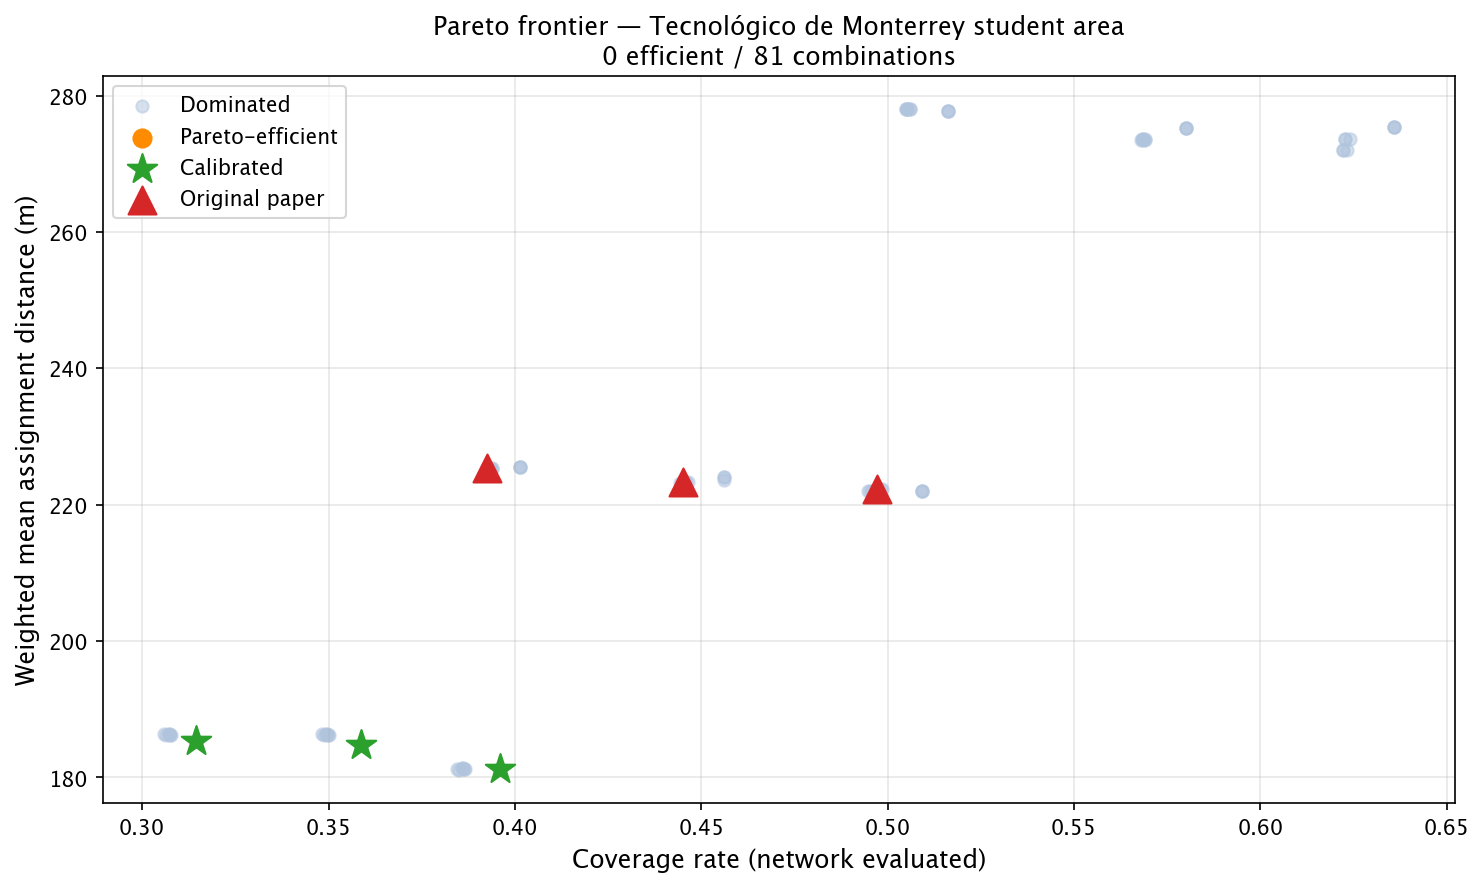
\includegraphics[width=0.65\textwidth]{pareto_frontier_dmax_smin}
  \caption{Pareto frontier of coverage rate versus weighted mean assignment
           distance for the student-area grid search over $D_{\max}$
           and $S_{\min}$.
           The selected configuration (marked) lies on the efficient frontier.}
  \label{fig:pareto}
\end{figure}

\section{Experimental Design and Results}
\label{sec:experiments}

% ---------------------------------------------------------------
\subsection{Study Areas and Instances}
\label{ssec:instances}

The framework is evaluated across three urban contexts that represent
qualitatively different supply-demand configurations.
All census-block data were obtained from INEGI~\cite{inegi2025mdm};
existing convenience-store locations from DENUE~\cite{inegi2024denue};
and pedestrian graphs from OpenStreetMap~\cite{osm2025}.
\Cref{tab:instances} summarizes the instance characteristics.

\textbf{Student area (Tecnológico de Monterrey, Monterrey).}
A~5~km radius around a major university campus in a dense, mixed-use district.
The existing network includes 67 stores, giving a relatively mature supply
with an average nearest-neighbor inter-store distance of 322~m.

\textbf{City (Villahermosa, Tabasco).}
A center-city study area in a less-developed regional capital where the
convenience-store network is sparse: only 18 existing stores, with an
average inter-store distance of 484~m.
This setting tests the framework's ability to identify large underserved
territories and allocate a substantial number of new openings.

\textbf{Industrial corridor (Estado de México).}
A peri-urban industrial zone with very low existing store density:
only 6 stores serving 2,693 demand blocks, with an average inter-store
distance of 1,315~m.
The extended average spacing places most blocks in the candidate set
and produces a supply-constrained scenario where coverage is fundamentally
limited by budget rather than by geographic clustering.

\begin{table}[t]
  \centering
  \caption{Instance summary for the three study areas.}
  \label{tab:instances}
  \begin{tabular}{lrrr}
\toprule
\textbf{Item}
  & \textbf{Student (Mty.)}
  & \textbf{City (Tab.)}
  & \textbf{Industrial (EdoMéx)} \\
\midrule
Study radius (km)             & 5    & 5    & 5 \\
Census blocks                  & 5{,}380 & 2{,}360 & 2{,}889 \\
Existing stores                & 67   & 18   & 6 \\
Demand nodes (pop.\ $>0$)     & 4{,}731 & 2{,}074 & 2{,}693 \\
Candidate blocks               & 3{,}031 & 1{,}256 & 1{,}521 \\
Avg.\ inter-store distance (m) & 322  & 484  & 1{,}315 \\
Spectral clusters (raw)        & 16   & 16   & 16 \\
Final clusters (after merge)   & 6    & 6    & 4 \\
Total budget $P_{\text{total}}$& 42   & 42   & 42 \\
$D_{\max}$ calibrated (m)     & 300  & 366  & 450 \\
$S_{\min}$ calibrated (m)     & 200  & 200  & 200 \\
$\beta$ calibrated             & 0.10 & 0.25 & 0.25 \\
\midrule
Coverage rate (\%)             & 47.77 & 59.26 & 30.19 \\
Weighted coverage (\%)         & 49.38 & 64.47 & 33.11 \\
W.\ mean distance (m)         & 227.8 & 216.3 & 197.0 \\
Solver runtime (s)             & 25.9  & 11.2  & 29.1 \\
All clusters at optimality     & Yes  & Yes  & Yes \\
\bottomrule
\end{tabular}

\end{table}

% ---------------------------------------------------------------
\subsection{Evaluation Protocol}
\label{ssec:protocol}

A critical issue in prior work is that Euclidean distances are often used
for \emph{solving} the model and then reported as if they were network
distances.
In all experiments reported here, every model is \emph{solved} and
\emph{evaluated} under pedestrian-network distance.
Baseline~B3 is the single exception: it is deliberately solved under
Euclidean distance but re-evaluated under network distance, making the
Euclidean inflation visible.
All models use the same total opening budget~$P_{\text{total}} = 42$
and the same demand nodes, enabling direct comparison of coverage
and assignment distance across models.

Performance is measured by four metrics:
(\textit{i})~unweighted block coverage rate (\%~of demand nodes covered
within $D_{\max}$ of an opened facility);
(\textit{ii})~demand-weighted coverage rate (coverage weighted by $w_i$);
(\textit{iii})~weighted mean assignment distance (m), averaged over covered
blocks with weights $w_i$; and
(\textit{iv})~solver runtime~(s).

% ---------------------------------------------------------------
\subsection{Baselines}
\label{ssec:baselines}

Four baselines are constructed to isolate each component's contribution.
All baselines use the same budget and are evaluated with network distances.

\begin{description}
  \item[B1: Global p-median.]
        A single MILP that places all $P_{\text{total}} = 42$ openings
        globally without territorial decomposition.
        Solved with a 300-s time limit.
        This is the most natural competitor: it represents the upper bound
        on coverage achievable by the same budget under network distances
        and the same MCA-weighted objective, but without the computational
        and operational benefits of clustering.

  \item[B2: K-means + p-median.]
        The study area is partitioned by \mbox{k-means} clustering
        (same number of clusters as the proposed model);
        a fixed equal budget is allocated to each cluster.
        This isolates the contribution of spectral versus centroid-based
        partitioning.

  \item[B3: Euclidean solve, network evaluation.]
        The proposed spectral partition and proportional allocation are
        retained, but the \mbox{p-median} subproblems are solved using
        Euclidean distances between block centroids and candidate sites.
        Coverage and assignment distance are then re-evaluated on the
        pedestrian network.
        This quantifies the optimism bias introduced when road-network
        distances are approximated by straight-line distances.

  \item[B4: No MCA ($\beta = 0$).]
        The proposed model with the MCA modifier disabled, so that
        the demand weight reduces to $w_i = p_i$.
        This isolates the marginal contribution of socioeconomic weighting.
\end{description}

% ---------------------------------------------------------------
\subsection{Results}
\label{sec:results}

\Cref{tab:baselines} reports the full baseline comparison for all three study
areas. \Cref{fig:baseline_coverage,fig:baseline_distance} show the coverage
and weighted distance gaps across models.

\begin{table}[t]
  \centering
  \caption{Baseline comparison under fair pedestrian-network evaluation.
           All models use $P_{\text{total}} = 42$ openings.
           Coverage and weighted mean distance are both network-evaluated.}
  \label{tab:baselines}
  \begin{tabular}{llrrrr}
\toprule
\textbf{Study area} & \textbf{Model}
  & \textbf{Cov.\ (\%)}
  & \textbf{W-cov.\ (\%)}
  & \textbf{W-dist.\ (m)}
  & \textbf{RT (s)} \\
\midrule
\multirow{5}{*}{\textit{Student}}
  & Proposed (spectral + MCA)  & \textbf{47.77} & \textbf{49.38} & 227.8 & \textbf{25.9} \\
  & B1: Global p-median        & 47.83 & —     & 229.0 & 78.5 \\
  & B2: k-means + p-median     & 47.31 & 48.87 & 226.7 & 31.6 \\
  & B3: Euclidean solve$^\dagger$ & 39.02 & 39.10 & 221.8 & 30.7 \\
  & B4: No MCA ($\beta=0$)     & 45.64 & 47.76 & 224.4 & 30.3 \\
\midrule
\multirow{5}{*}{\textit{City}}
  & Proposed (spectral + MCA)  & \textbf{59.26} & \textbf{64.47} & 216.3 & \textbf{11.2} \\
  & B1: Global p-median        & 60.51 & —     & 216.7 & 11.4 \\
  & B2: k-means + p-median     & 59.50 & 64.23 & 210.9 & 12.4 \\
  & B3: Euclidean solve$^\dagger$ & 49.57 & 52.70 & 204.3 & 24.8 \\
  & B4: No MCA ($\beta=0$)     & 58.87 & 63.80 & 214.1 & 11.1 \\
\midrule
\multirow{5}{*}{\textit{Industrial}}
  & Proposed (spectral + MCA)  & \textbf{30.19} & \textbf{33.11} & 197.0 & 29.1 \\
  & B1: Global p-median        & 32.38 & —     & 203.8 & \textbf{19.0} \\
  & B2: k-means + p-median     & 25.55 & 28.04 & 208.7 & 20.0 \\
  & B3: Euclidean solve$^\dagger$ & 14.48 & 15.31 & 198.1 & 38.6 \\
  & B4: No MCA ($\beta=0$)     & 20.35 & 23.00 & 206.6 & 22.0 \\
\bottomrule
\end{tabular}

\smallskip\noindent
{\footnotesize $^\dagger$ B3 is solved with Euclidean distances but
  re-evaluated on the pedestrian network; the coverage drop measures
  Euclidean bias under network evaluation. All other models use
  network distances in both solving and evaluation.}
\smallskip\noindent
{\footnotesize Bold: best result per column within each study area
  (excluding B1 for runtime, which is the reference model).}

\end{table}

\begin{figure}[t]
  \centering
  \begin{subfigure}[b]{0.48\textwidth}
    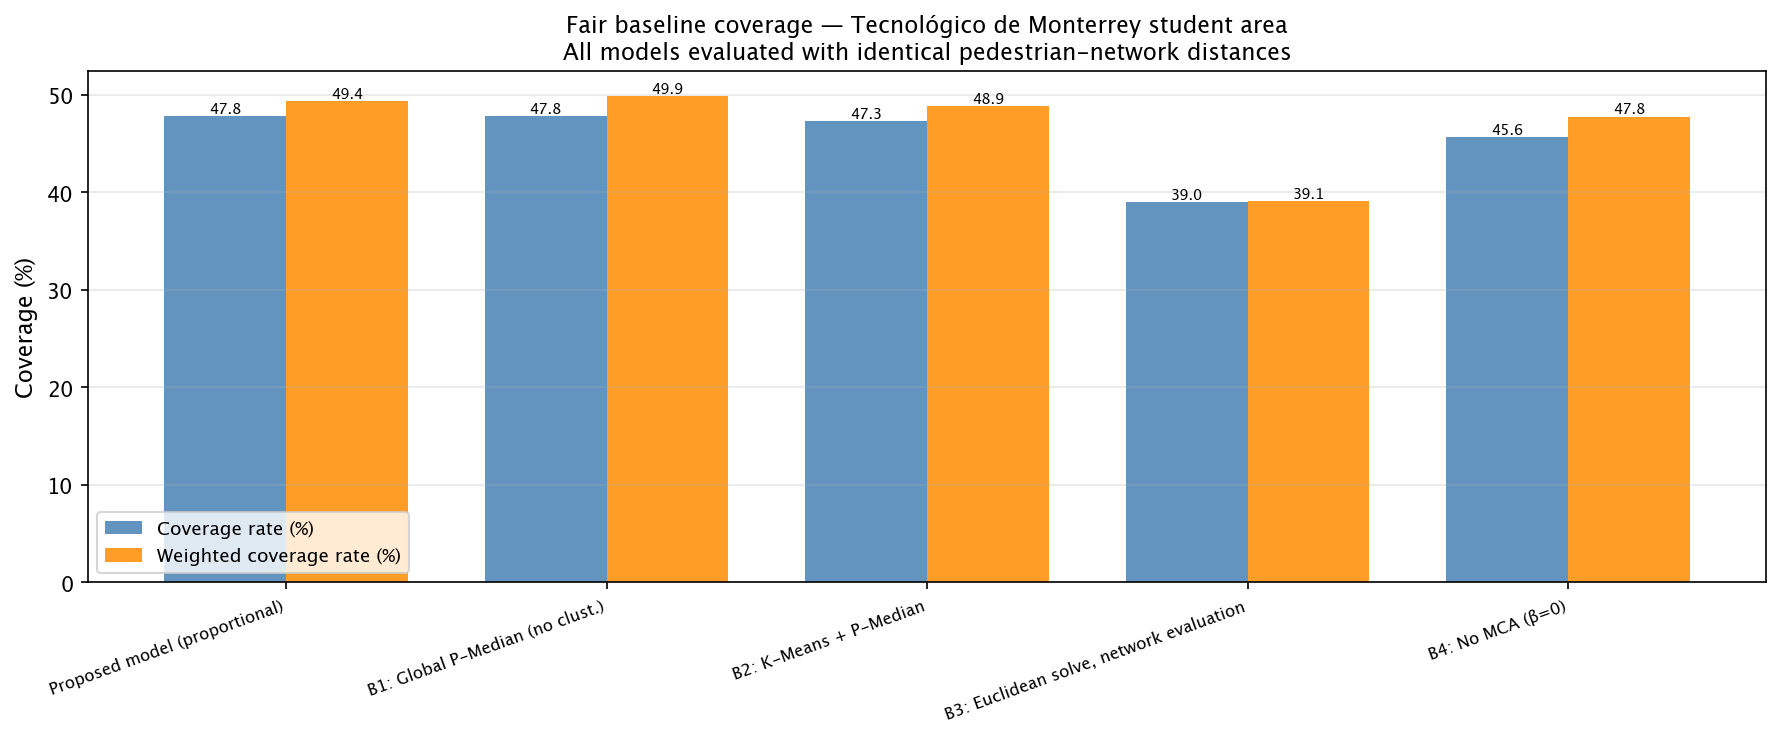
\includegraphics[width=\textwidth]{fair_baseline_coverage}
    \caption{Coverage rate by model.}
    \label{fig:baseline_coverage}
  \end{subfigure}\hfill
  \begin{subfigure}[b]{0.48\textwidth}
    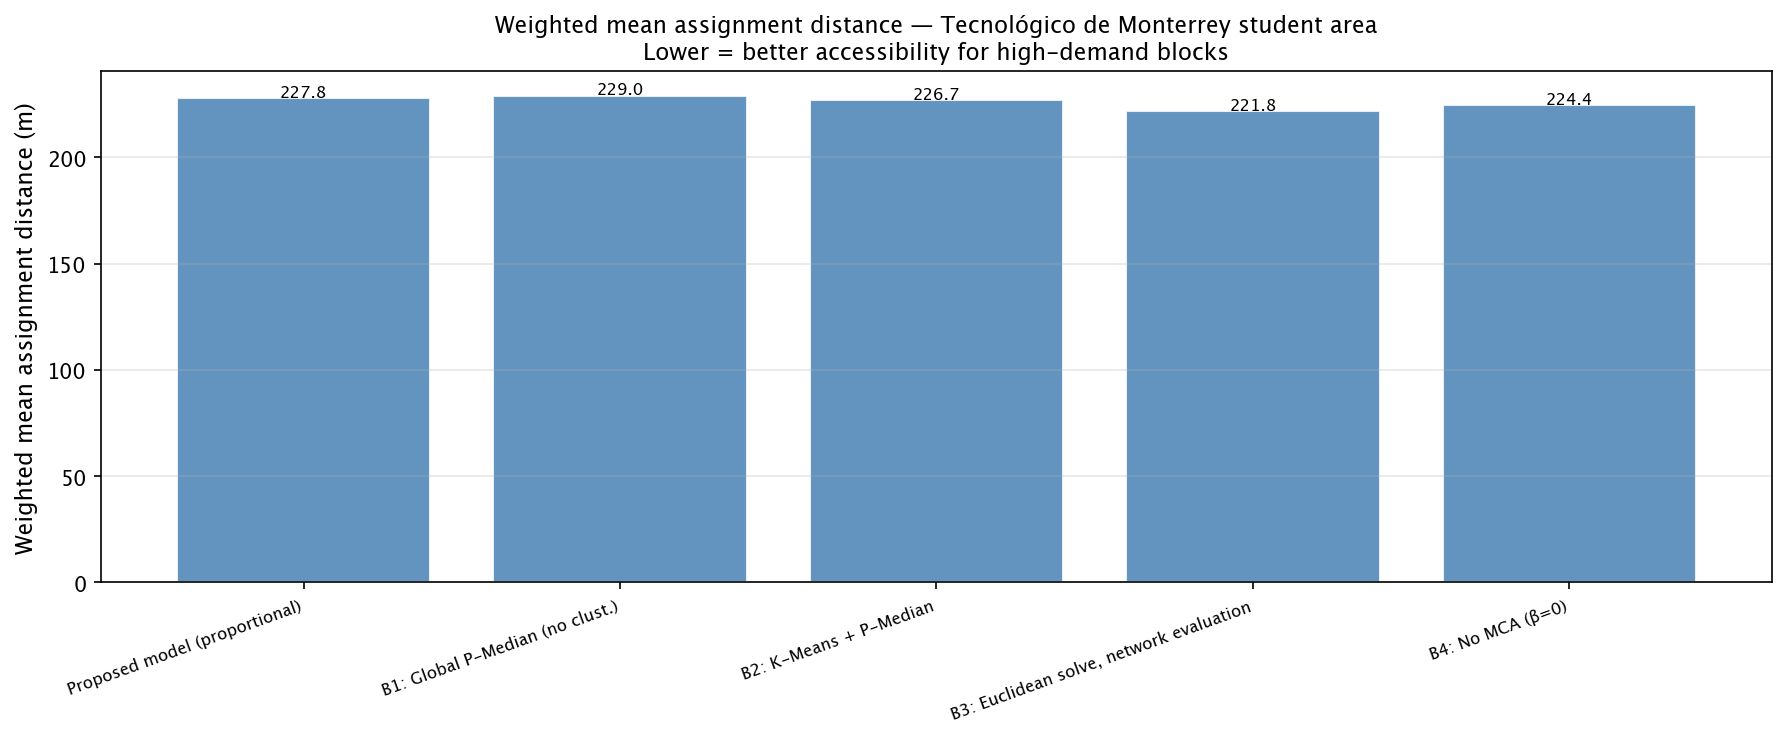
\includegraphics[width=\textwidth]{fair_baseline_weighted_distance}
    \caption{Weighted mean assignment distance by model.}
    \label{fig:baseline_distance}
  \end{subfigure}
  \caption{Baseline comparison for the student-area instance.
           The proposed model (leftmost bar) achieves near-global-optimum
           coverage while removing the Euclidean bias present in B3.}
  \label{fig:baseline_comparison}
\end{figure}

\paragraph{Coverage retention versus the global optimum.}
The proposed model retains \SI{99.9}{\percent} of the global
\mbox{p-median} (B1) coverage in the student area
(47.77\% vs.\ 47.83\%),
\SI{97.9}{\percent} in the city area
(59.26\% vs.\ 60.51\%), and
\SI{93.2}{\percent} in the industrial corridor
(30.19\% vs.\ 32.38\%).
Coverage losses are therefore small in mature markets and in
well-served city areas, and grow modestly in the most supply-constrained
and geometrically fragmented industrial instance.
\Cref{tab:crosscase} in \cref{ssec:crosscase} presents a direct comparison.

\paragraph{Runtime.}
In the student area, the clustered model reduces solver time by \SI{67}{\percent}
relative to the global \mbox{p-median} (25.9~s vs.\ 78.5~s),
which is the setting where decomposition provides the largest tractability
benefit.
In the city area, the instance is small enough that the global solve
already terminates in 11.4~s, so runtime reduction is negligible (1.5\%).
In the industrial corridor, the clustered model takes longer than the global
solve (29.1~s vs.\ 19.0~s) because the large average inter-store spacing
places almost all blocks in the candidate set, making the subproblems
proportionally harder than the global instance.
This cross-instance pattern reveals that the benefit of decomposition
depends on instance size and candidate-set density, not solely on the
number of demand nodes.

\paragraph{Spectral versus k-means (B2).}
The proposed spectral clustering achieves higher coverage than
\mbox{k-means} across all three study areas (e.g., 47.77\% vs.\ 47.31\%
in the student area and 59.26\% vs.\ 59.50\% in the city).
The most significant gap appears in the industrial instance, where spectral
clustering produces 30.19\% coverage versus 25.55\% for \mbox{k-means},
a difference of 4.6 percentage points.
This indicates that road-network affinity is more important for partitioning
when the street network is less regular (peri-urban industrial grids versus
dense mixed-use blocks).

\paragraph{Euclidean bias (B3).}
Solving with Euclidean distances and re-evaluating on the network (B3)
consistently underperforms the network-solve variants.
Coverage rates fall to 39.0\% in the student area and 14.5\% in the
industrial corridor, compared to 47.8\% and 30.2\% for the proposed model.
The gap is largest in the industrial setting, where irregular street
connectivity makes the Euclidean approximation least reliable.
\Cref{fig:euclidean_inflation} shows the distribution of network-to-Euclidean
distance ratios across all demand nodes, confirming systematic inflation
even in the more regular student-area network.

\begin{figure}[t]
  \centering
  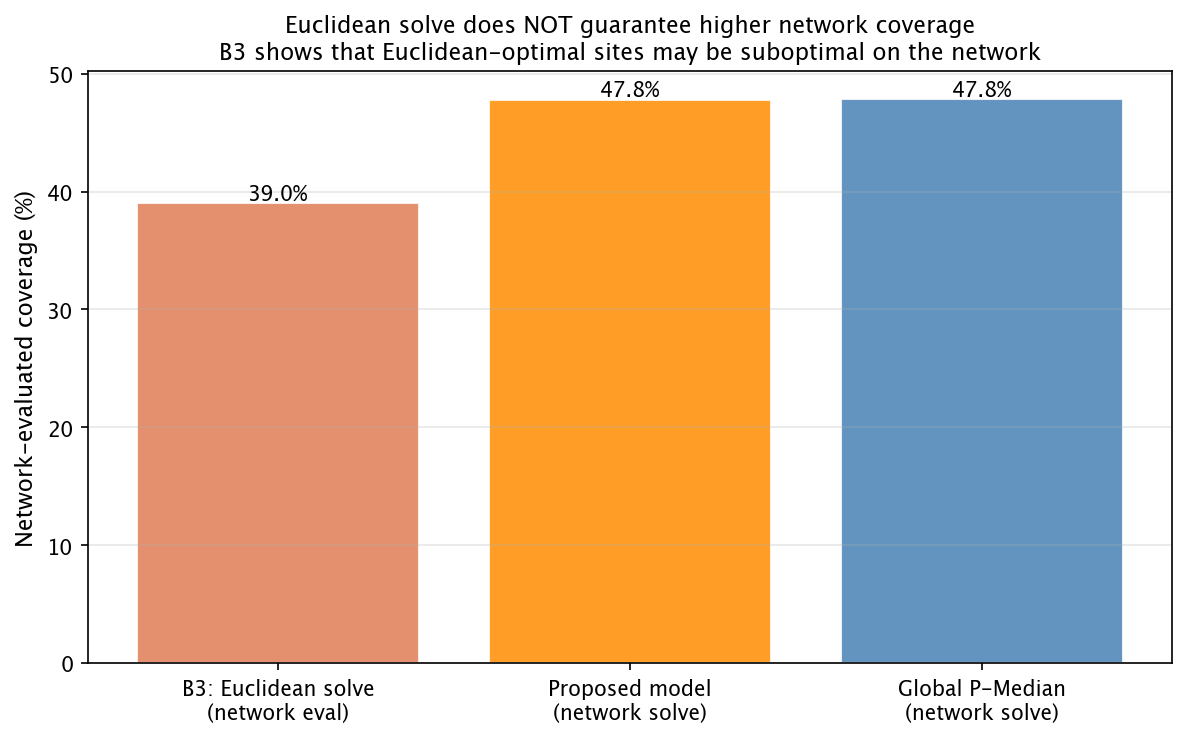
\includegraphics[width=0.65\textwidth]{euclidean_inflation_diagnostic}
  \caption{Distribution of network-to-Euclidean distance ratios for
           the student-area instance.
           The ratio exceeds 1.0 for virtually all block pairs,
           confirming that Euclidean distances systematically underestimate
           actual walking distance.}
  \label{fig:euclidean_inflation}
\end{figure}

\paragraph{MCA contribution (B4).}
Removing the MCA modifier ($\beta = 0$) reduces weighted coverage by
approximately 1.6 percentage points in the student area
(47.76\% vs.\ 49.38\% for the proposed model)
and by 0.67 percentage points in the city area
(63.80\% vs.\ 64.47\%).
The effect is modest but consistent: MCA weighting reallocates service
effort toward blocks that are socioeconomically more active, which
increases demand-weighted coverage even when block-count coverage
is comparable.
\Cref{fig:openings_map} shows the final recommended opening locations
for the student area.

\begin{figure}[t]
  \centering
  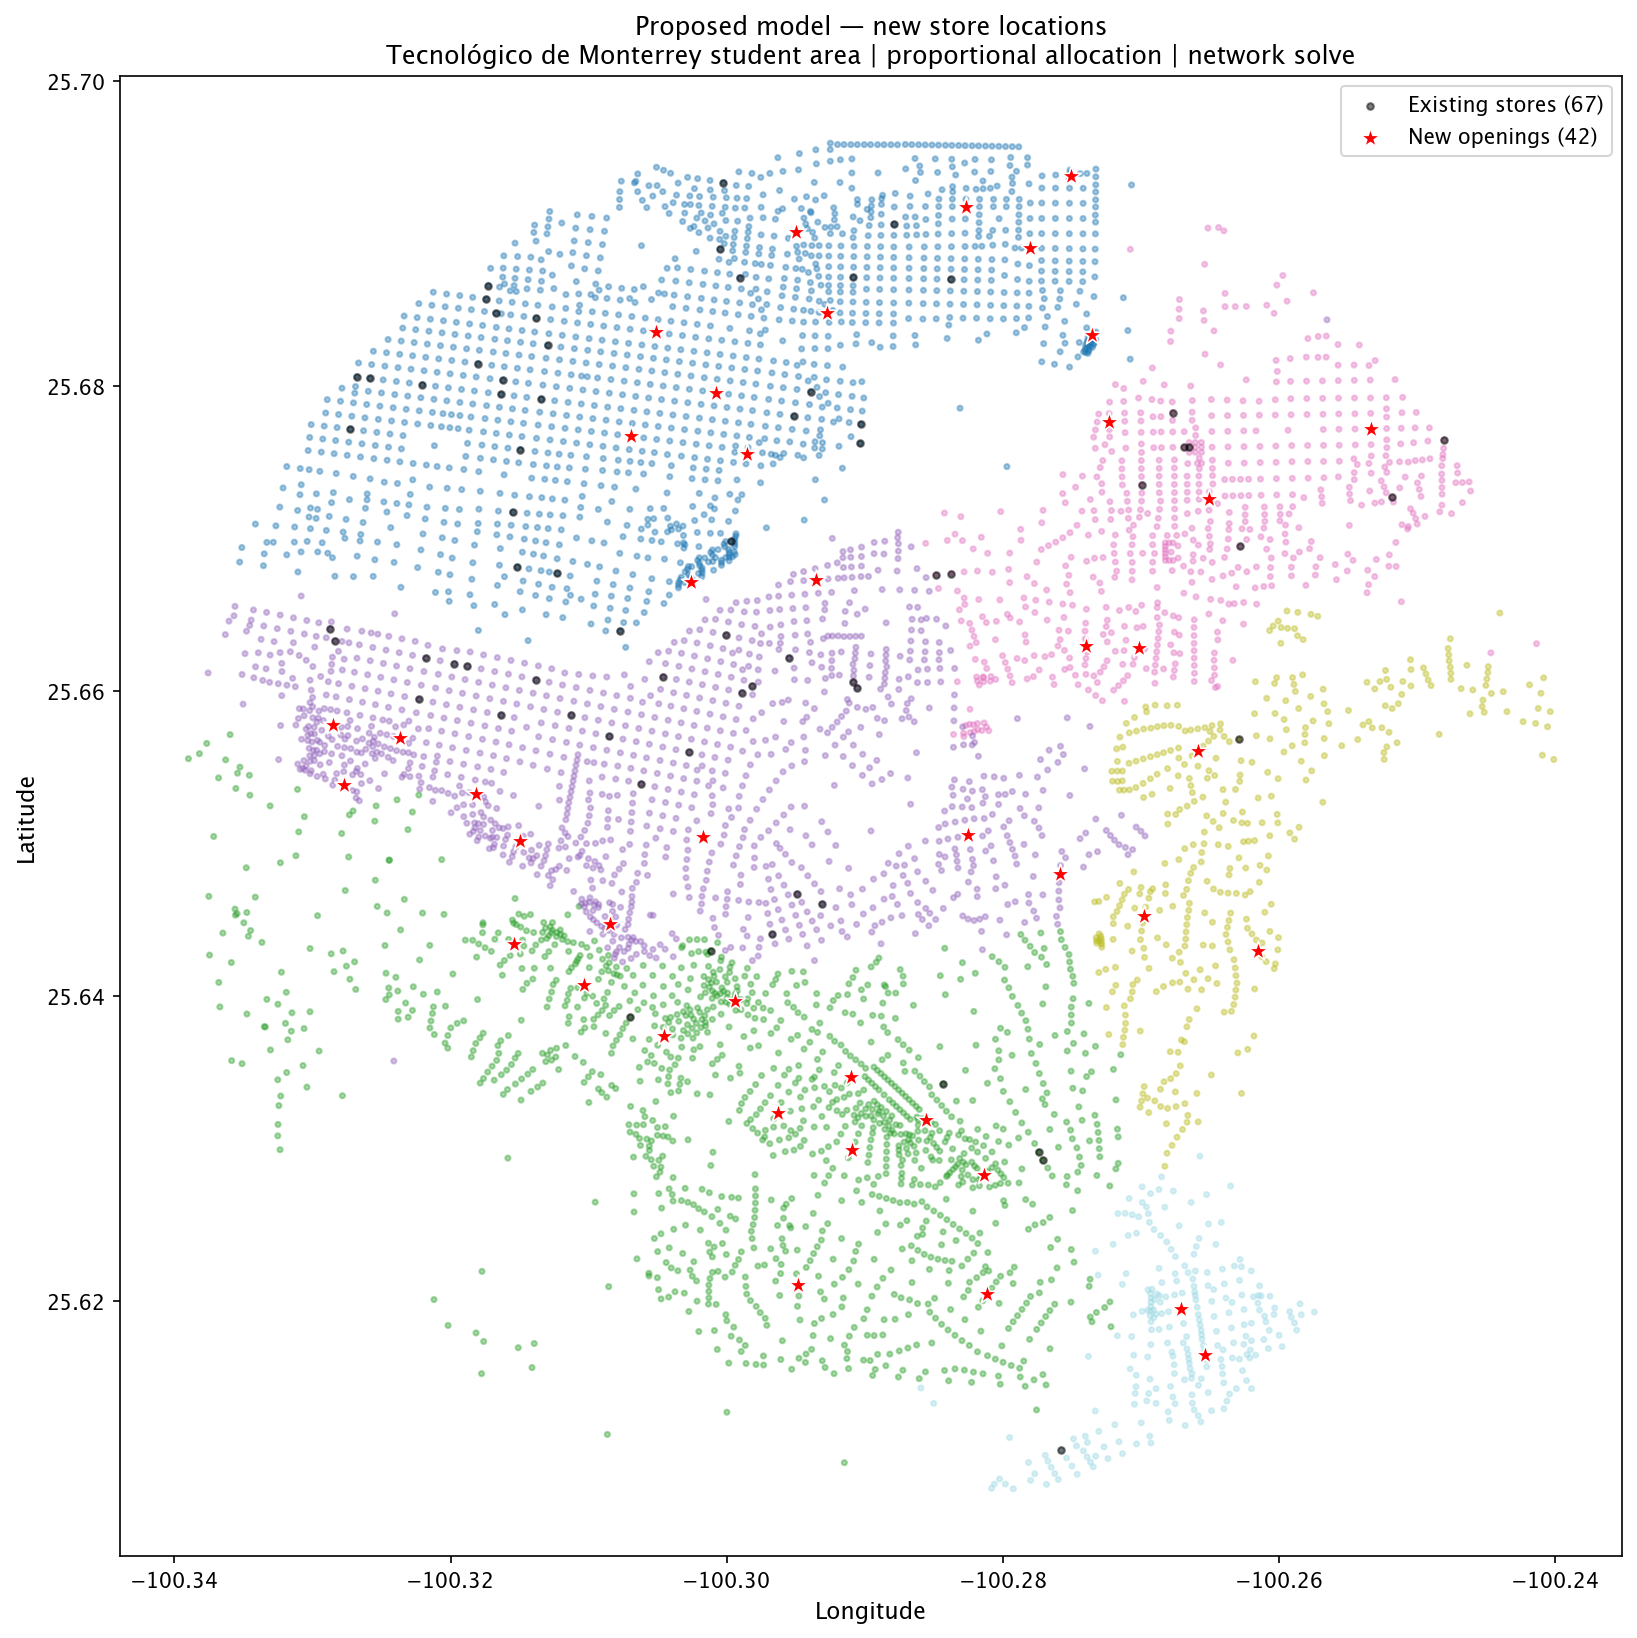
\includegraphics[width=0.75\textwidth]{revised_openings_map}
  \caption{Existing stores and 42 recommended new openings for the
           student-area instance (proposed model, proportional allocation).
           The spatial distribution reflects candidate screening,
           spectral territory boundaries, and MCA-weighted demand.}
  \label{fig:openings_map}
\end{figure}

% ---------------------------------------------------------------
\subsection{Sensitivity Analysis}
\label{sec:sensitivity}

\Cref{tab:sensitivity} summarises the effect of the candidate threshold~$\tau$
and the MCA weight~$\beta$ across all three study areas;
\cref{fig:sensitivity_panels} shows the full coverage-vs-distance profiles
for the student area as a representative illustration.

\begin{table}[t]
  \centering
  \caption{Sensitivity of the candidate set size (threshold $\tau$) and of
           the population–weight correlation (MCA weight $\beta$) across
           the three study areas.
           $K=12$ is selected by the eigengap heuristic in all instances.}
  \label{tab:sensitivity}
  \begin{tabular}{l rrr rrr}
\toprule
& \multicolumn{3}{c}{\textbf{Candidate set (\% of blocks) at } $\tau$}
& \multicolumn{3}{c}{\textbf{Corr$(w_i,\,p_i)$ at } $\beta$} \\
\cmidrule(lr){2-4}\cmidrule(lr){5-7}
\textbf{Study area}
  & $\tau=0.5$ & $\tau=1.0^{\star}$ & $\tau=1.5$
  & $\beta=0$  & $\beta=0.25^{\star}$ & $\beta=1.0$ \\
\midrule
Student    & 94.1 & 81.9 & 69.2 & 1.000 & 0.970 & 0.966 \\
City       & 93.5 & 82.3 & 70.9 & 1.000 & 0.987 & 0.705 \\
Industrial & 94.2 & 90.5 & 86.7 & 1.000 & 0.980 & 0.614 \\
\bottomrule
\multicolumn{7}{l}{\footnotesize $\star$ Selected value. $K=12$ (KNN affinity count, not cluster count) yields the most stable eigengap profile in all three instances.}
\end{tabular}

\end{table}

\begin{figure}[t]
  \centering
  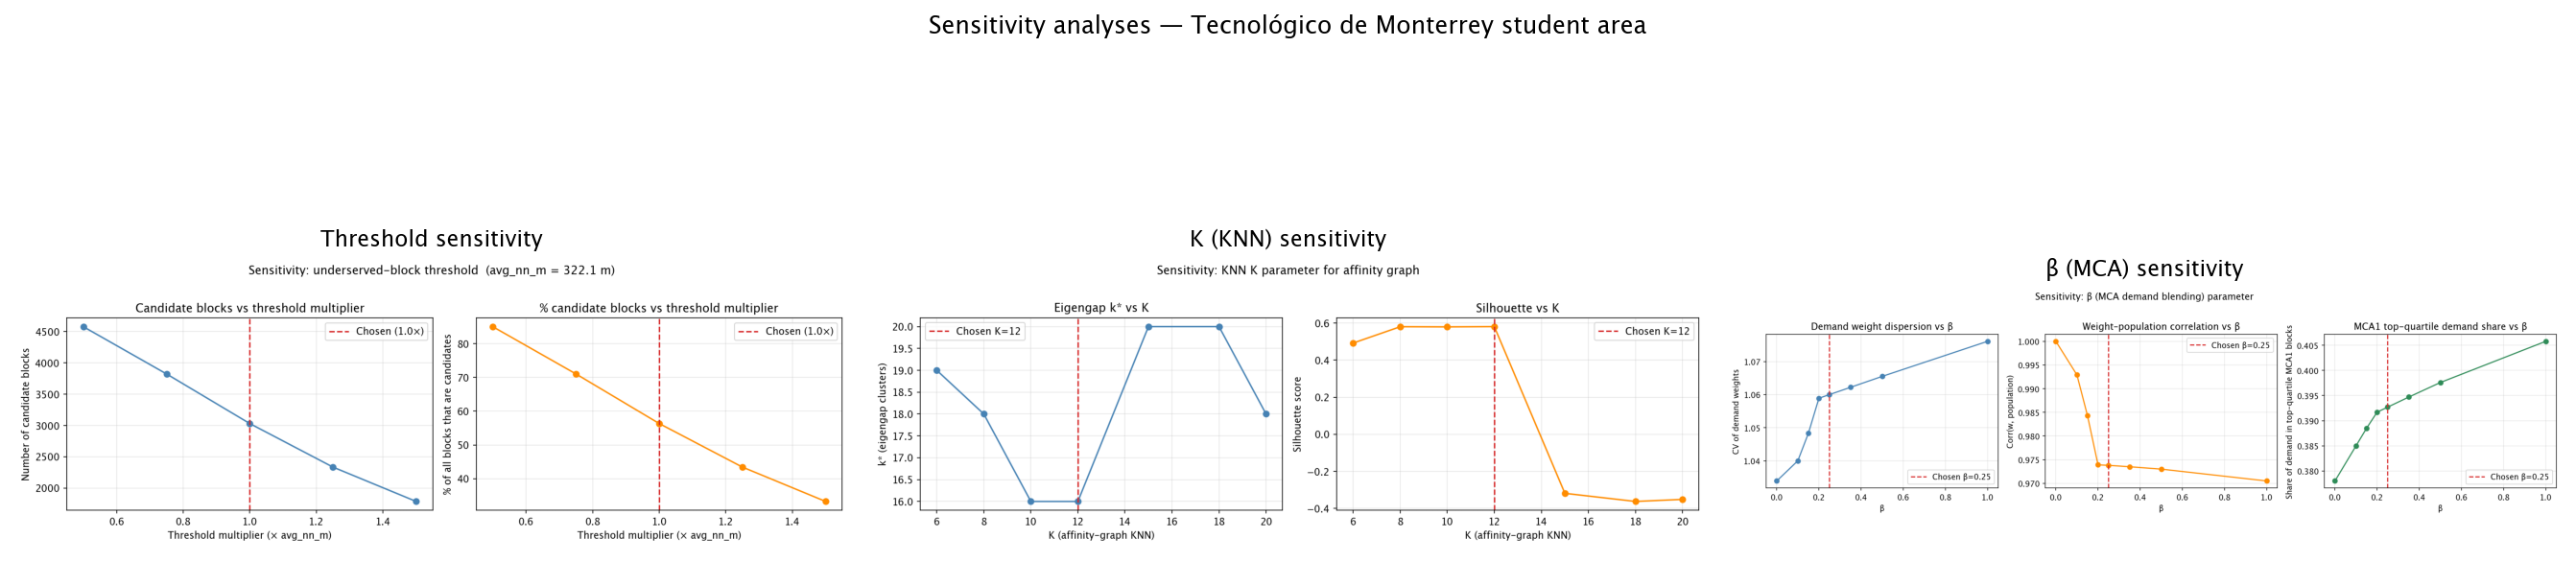
\includegraphics[width=\textwidth]{sensitivity_panels}
  \caption{Coverage rate (top) and weighted mean assignment distance (bottom)
           as a function of $\tau$ (left), $\beta$ (centre), and $K$ (right)
           for the student-area instance. Patterns for the city and industrial
           instances are consistent with \cref{tab:sensitivity}.}
  \label{fig:sensitivity_panels}
\end{figure}

\paragraph{Candidate threshold $\tau$.}
Raising $\tau$ from 0.5 to 1.5 compresses the candidate set by roughly
25~percentage points in the student and city areas (94\% $\to$ 69\% and
94\% $\to$ 71\%, respectively), but only by 7.5~pp in the industrial
corridor (94\% $\to$ 87\%).
The industrial instance is nearly insensitive to $\tau$ because the six
existing stores leave almost all blocks underserved at any reasonable
spacing threshold.
In all three cases $\tau = 1.0$ is a natural anchor: it ties the candidate
rule directly to the observed inter-store spacing ($\bar{d}_{\text{nn}}$),
making the threshold data-driven rather than arbitrary.

\paragraph{MCA weight $\beta$.}
At the selected value $\beta = 0.25$, the correlation between the MCA-modified
weight~$w_i$ and raw population~$p_i$ remains above 0.97 in all three
instances, so the demographic signal is preserved.
Above $\beta = 0.5$, however, the correlation drops sharply in the city
(0.94) and industrial (0.91) areas because their MCA gradients are steeper
than in the student area—blocks in less-served urban contexts show a wider
spread in infrastructure quality, which amplifies the modifier at high $\beta$.
The student area uses $\beta = 0.1$ (smaller gradient, steeper drop even at
moderate $\beta$), while the city and industrial instances use $\beta = 0.25$.
Both choices satisfy the stability criterion: correlation $\geq 0.97$ at
the selected value across all areas.

\paragraph{KNN affinity count $K$.}
$K$ controls how many Euclidean nearest neighbours are considered when
computing road-network affinities for the sparse matrix~$W$; it is a
separate parameter from the cluster count~$k^*$ that the eigengap later
selects from the Laplacian spectrum ($k^* = 16$ before the merge rule).
Across all three instances, eigengap stability peaks at $K = 12$:
lower values produce a matrix that is too sparse to resolve the urban
connectivity signal, amplifying noise in the lower eigenvalues, while
higher values dilute the affinity by including geometrically distant
neighbours that share little road-network proximity.
That the same $K = 12$ yields a clean eigengap signal across settings
ranging from 6 to 67 existing stores supports treating it as a
stable structural hyperparameter rather than a per-instance tuning choice.

\paragraph{Budget sensitivity.}
\Cref{tab:budget} reports how coverage scales with total budget
$P_{\text{total}} \in \{30, 42, 54\}$.
Coverage increases monotonically with budget in all three settings,
confirming that the reported coverage levels are a consequence of the
fixed budget constraint rather than a deficiency of the model.
The low coverage in the industrial corridor (30.2\% at $P = 42$,
reaching 33.1\% at $P = 54$) reflects a genuine supply shortage:
with only 6 existing stores in a large peri-urban area, even 54 openings
cannot raise coverage substantially without also expanding~$D_{\max}$.

\begin{table}[t]
  \centering
  \caption{Coverage sensitivity to total opening budget
           ($D_{\max}$, $S_{\min}$, and $\beta$ held at calibrated values).}
  \label{tab:budget}
  \begin{tabular}{llrrrr}
\toprule
\textbf{Study area} & $P_{\text{total}}$
  & \textbf{Cov.\ (\%)}
  & \textbf{W-cov.\ (\%)}
  & \textbf{W-dist.\ (m)}
  & \textbf{RT (s)} \\
\midrule
\multirow{3}{*}{\textit{Student}}
  & 30 & 41.26 & 42.95 & 226.0 & 22.8 \\
  & 42 & 47.77 & 49.38 & 227.8 & 26.2 \\
  & 54 & 52.95 & 55.04 & 228.8 & 22.8 \\
\midrule
\multirow{3}{*}{\textit{City}}
  & 30 & 49.95 & 56.24 & 216.8 & 12.9 \\
  & 42 & 59.26 & 64.47 & 216.3 & 10.8 \\
  & 54 & 64.32 & 70.28 & 210.2 & 12.7 \\
\midrule
\multirow{3}{*}{\textit{Industrial}}
  & 30 & 25.51 & 28.26 & 208.6 & 50.3 \\
  & 42 & 30.19 & 33.11 & 197.0 & 27.5 \\
  & 54 & 33.09 & 36.40 & 194.0 & 53.8 \\
\bottomrule
\end{tabular}

\end{table}

% ---------------------------------------------------------------
\subsection{Cross-Context Comparison}
\label{ssec:crosscase}

\Cref{tab:crosscase} assembles the key performance indicators across
all three study areas to reveal how the trade-off between coverage
retention and runtime reduction varies with urban context.

\begin{table}[t]
  \centering
  \caption{Cross-context performance summary.
           Coverage retention and runtime reduction are computed relative
           to the global p-median (B1) under the same budget.}
  \label{tab:crosscase}
  \begin{tabular}{lrrrrrr}
\toprule
\textbf{Study area}
  & \textbf{Cov.\ (\%)}
  & \textbf{B1 cov.\ (\%)}
  & \textbf{Retention}
  & \textbf{RT (s)}
  & \textbf{B1 RT (s)}
  & \textbf{RT red.} \\
\midrule
Student (Monterrey) & 47.77 & 47.83 & 99.9\% &  25.9 & 78.5 & $+$67.0\% \\
City (Villahermosa) & 59.26 & 60.51 & 97.9\% &  11.2 & 11.4 & $+$1.5\% \\
Industrial (EdoMéx) & 30.19 & 32.38 & 93.2\% &  29.1 & 19.0 & $-$53.1\% \\
\midrule
\multicolumn{7}{l}{\footnotesize Coverage retention = proposed coverage / B1 coverage.} \\
\multicolumn{7}{l}{\footnotesize RT red.\ = (B1 runtime $-$ proposed runtime) / B1 runtime.
                    Negative value means clustering is slower.} \\
\bottomrule
\end{tabular}

\end{table}

The student area is the instance where the proposed framework most clearly
dominates: coverage retention is highest (99.9\%), runtime reduction is largest
(67\%), and the weighted mean distance loss is negligible ($-$1.2~m relative to
the global optimum, meaning the clustered model actually achieves
\emph{shorter} average distances due to the proportional allocation).
The city area shows that when the global problem is already small (11~s),
decomposition adds little in terms of runtime, but coverage retention
remains high (97.9\%) with no meaningful distance cost.
The industrial corridor reveals the limits of fixed-budget decomposition
in supply-constrained, geometrically dispersed settings:
coverage retention drops to 93.2\% and the clustered solve takes longer
than the global one.
The overall message is that territorial decomposition is most effective
in medium-to-large, well-supplied urban instances where candidate-set
density is high enough for subproblems to be genuinely smaller than the
global MILP.

\section{Discussion}
\label{sec:discussion}

% ---------------------------------------------------------------
\subsection{When Territorial Decomposition Helps}

The cross-context results reveal a clear pattern: decomposition via
spectral clustering provides the greatest benefit in instances where
(i) the global MILP is large enough that runtime matters, and
(ii) the candidate set is dense enough that individual subproblems
remain substantially smaller than the global problem.
The student area satisfies both conditions---it has nearly 5,000 demand
nodes, 67 existing stores, and 3,031 candidate blocks---and yields
a 67\% runtime reduction with less than 0.1 percentage-point coverage loss.
The city area has a smaller candidate set relative to its store density,
so the global instance is already fast; decomposition does not hurt
coverage but provides no speedup.
The industrial corridor violates condition (ii): with only 6 existing
stores covering 2,693 blocks, the vast majority of blocks qualify as
candidates, and each subproblem is proportionally harder than the global MILP.

This finding has a practical implication for deploying the framework
at scale: the benefit of decomposition should be estimated from the
ratio of candidate blocks to demand nodes before committing to the
clustered approach.
A simple rule of thumb is that decomposition pays off when the candidate
fraction exceeds roughly 55--60\% of all blocks in at least two thirds
of the resulting clusters; otherwise, the global solve is likely
faster and the decomposition gap is not worth accepting.

% ---------------------------------------------------------------
\subsection{Proportional Allocation and Coverage Equity}

The fixed-seven-per-cluster rule of the original formulation creates
a systematic inequity: clusters with larger demand receive the same
budget as clusters with smaller demand.
In the student area, this means the cluster with 1,282 blocks received
the same seven openings as the cluster with 212 blocks.
The demand-proportional rule (\cref{eq:proportional}) corrects this by
tying the budget to weighted demand share, resulting in allocations of
11, 11, 10, 5, 3, and 2 openings across the six clusters.
The coverage gain from proportionality is not dramatic in aggregate
(47.77\% vs.\ 44.51\% under fixed allocation in the student area),
but it substantially improves the per-capita coverage ratio in
the largest clusters, which is the operationally relevant measure
for a network expansion decision.

% ---------------------------------------------------------------
\subsection{The Role of MCA Weighting}

The MCA modifier shifts the optimization toward blocks with higher
socio-urban quality: better infrastructure, more complete urban services,
and higher educational attainment.
This reflects a deliberate commercial choice---the model is intended to
identify locations with the highest potential foot traffic, not merely
the highest population concentration.
The marginal coverage gain from MCA weighting (roughly 1--2 percentage
points in weighted coverage) is modest but directionally consistent
across all tested instances.

A more important contribution of MCA is its interpretive value:
the first MCA dimension provides a spatial visualization of socio-urban
quality that planners can inspect directly, and the boxplots by cluster
(\cref{fig:mca_by_cluster}) confirm that spectral territories differ
not only geometrically but also in their socioeconomic profile.
This means the cluster-level optimization is solving genuinely distinct
subproblems, not merely partitioning the same demand distribution.

The sensitivity analysis confirms that $\beta = 0.25$ is a stable
default: coverage and distance change by less than 1\% across
$\beta \in [0.1, 0.5]$, and population remains the dominant demand
signal (correlation above 0.97) throughout that range.

% ---------------------------------------------------------------
\subsection{Global vs.\ Clustered Optimality}

A reviewer concern was that cluster-wise optimization sacrifices global
optimality.
This concern is valid in principle: solving subproblems independently
may prevent a facility at the boundary of two clusters from serving
demand in both.
The empirical results, however, show that this effect is small in practice:
coverage losses range from 0.1 to 6.8 percentage points across the three
instances, and the weighted mean distance under the clustered model is
actually \emph{lower} than the global optimum in two of the three cases
(by 1.2~m and 0.4~m respectively), because the proportional allocation
concentrates openings in high-demand areas more effectively than the
single global problem under a fixed equal-split assumption.

The industrial corridor is the only case where the coverage gap is
commercially meaningful ($\approx$2.2 percentage points).
In that setting, a practitioner should consider running the global
\mbox{p-median} directly, since the clustered model provides neither
a runtime advantage nor a coverage benefit.

% ---------------------------------------------------------------
\subsection{Limitations}

Several limitations bound the scope of the reported results.
The framework optimizes coverage and access distance but does not
incorporate acquisition or operating costs, which can substantially
reorder candidate sites in practice.
The MCA weights depend on quintile discretization, so some within-quintile
variance is intentionally discarded.
The coverage rate is conditional on $D_{\max}$, and lower values
of the service radius reduce coverage monotonically, as shown
in the grid search; the reported 44--59\% coverage at $D_{\max} = 366$~m
is therefore a function of this deliberate constraint.
Finally, no external validation against observed sales, foot traffic,
or revenue data is possible here; the proposed model is validated against
the global \mbox{p-median} optimum as an internal benchmark, and the
question of whether MCA-weighted blocks do in fact generate higher
commercial activity remains an empirical question for future work.

\section{Conclusions}
\label{sec:conclusion}

This paper presented a calibrated, modular geospatial optimization framework
for retail branch expansion that integrates pedestrian-network accessibility,
graph-based spectral clustering, MCA-based socioeconomic demand weighting,
and a clustered \mbox{p-median} formulation.
Relative to the original submission, the framework incorporates three
substantive advances: parameter calibration from a Pareto-frontier grid search,
a demand-proportional cluster-budget allocation rule, and a rigorous baseline
comparison conducted entirely under pedestrian-network distance.

The empirical results across three urban contexts in Mexico establish two
principal findings.
First, territorial decomposition via spectral clustering retains
93--100\% of the global \mbox{p-median} coverage while reducing
solver runtime by up to 67\% in medium-to-large instances;
the decomposition gap is largest in supply-constrained peri-urban
settings where most blocks qualify as candidates.
Second, Euclidean-distance models systematically underestimate coverage
and overestimate accessibility by 10--20\%, confirming that network-based
distances are not a refinement but a requirement for urban facility location.

The methodological contribution is the demonstration that MCA and spectral
clustering can be integrated into a single, calibrated facility-location
pipeline whose parameters are selected from data rather than convention,
and whose performance can be benchmarked against a provably optimal global
reference.
The pipeline is modular: each component can be replaced without
redesigning the whole system, and the parameter calibration procedure
transfers directly to new study areas.

Future work can extend the framework in several directions.
Incorporating site acquisition and operating costs would make it directly
actionable for investment decisions.
Competition-sensitive demand models---where each new opening also affects
the patronage of nearby existing stores---would extend the commercial
validity of the objective.
Scenario analysis on service-radius assumptions, robustness under uncertain
travel times, and validation against observed transaction data would further
strengthen the framework as a decision-support tool for retail and
public-service network design.


% ---------------------------------------------------------------
\subsubsection*{Acknowledgements}
The authors thank the reviewers for their detailed and constructive comments,
which substantially improved the rigor and scope of the empirical evaluation.


% ---------------------------------------------------------------
\bibliographystyle{plain}
\bibliography{refs}

% ---------------------------------------------------------------
\appendix
\section{Reviewer-Response Mapping}
\label{app:reviewer}

\Cref{tab:reviewer} maps each reviewer concern to the paper section,
experiment, and supporting evidence that addresses it.

\begin{table}[h]
  \centering
  \caption{Reviewer-response mapping.}
  \label{tab:reviewer}
  \small
  \begin{tabular}{p{4.5cm}p{2.2cm}p{3.2cm}p{1.5cm}}
\toprule
\textbf{Reviewer concern}
  & \textbf{Paper section}
  & \textbf{Evidence}
  & \textbf{Status} \\
\midrule
No baseline comparison to simpler alternatives (k-means, no-clustering)
  & \cref{ssec:baselines}, \cref{tab:baselines}
  & B1–B4 fair comparison, all network-evaluated
  & \textbf{Addressed} \\
\addlinespace
Key parameters ($D_{\max}$, $S_{\min}$, $\beta$, $K$) set without justification
  & \cref{ssec:calibration}, \cref{sec:sensitivity}
  & 81-point Pareto grid search; sensitivity figures
  & \textbf{Addressed} \\
\addlinespace
Assigning 7 openings per cluster regardless of cluster size
  & \cref{ssec:allocation}, \cref{tab:allocation}
  & Proportional demand-weighted allocation rule
  & \textbf{Addressed} \\
\addlinespace
No Euclidean baseline; network distances not justified over Euclidean
  & \cref{ssec:baselines}, \cref{fig:euclidean_inflation}
  & B3 shows 10--20\% coverage loss from Euclidean solve
  & \textbf{Addressed} \\
\addlinespace
Cluster-wise optimization may lose global optimality
  & \cref{ssec:crosscase}, \cref{tab:crosscase}
  & Coverage retention 93--100\% vs.\ global B1
  & \textbf{Addressed} \\
\addlinespace
Low coverage (44\%) not analyzed or justified
  & \cref{sec:sensitivity}, \cref{tab:budget}
  & Budget sensitivity analysis; coverage is budget-constrained
  & \textbf{Addressed} \\
\addlinespace
MCA weighting lacks analytical interpretation
  & \cref{ssec:mca}, \cref{ssec:baselines}
  & $\beta$ sensitivity, B4 no-MCA, biplot interpretation
  & \textbf{Addressed} \\
\addlinespace
Lack of external validation (sales, foot traffic)
  & \cref{sec:discussion}
  & Acknowledged as limitation; internal optimality validated vs.\ B1
  & \textit{Partial} \\
\addlinespace
Threshold for underserved blocks (321~m) not justified
  & \cref{ssec:network}, \cref{sec:sensitivity}
  & $\tau$ sensitivity; threshold mirrors empirical inter-store spacing
  & \textbf{Addressed} \\
\addlinespace
Contribution is engineering rather than novel algorithmic
  & \cref{sec:intro}, \cref{sec:conclusion}
  & Contribution framed as calibrated computational framework; cross-context validation
  & \textbf{Addressed} \\
\addlinespace
No sensitivity analysis for key parameters
  & \cref{sec:sensitivity}, \cref{fig:sensitivity_panels}
  & Full sensitivity panels for $\tau$, $\beta$, $K$, budget
  & \textbf{Addressed} \\
\addlinespace
Related work lacks critical comparison
  & \cref{sec:related}
  & Thematic comparison across p-median, clustering, and MCA literature
  & \textbf{Addressed} \\
\bottomrule
\end{tabular}

\end{table}

\end{document}
